\documentclass[hide notes,intlimits]{beamer}

\usepackage{tikz}
\usetikzlibrary{shapes,arrows}

\mode<presentation>
{
  \usetheme[footline]{UAFshade}
  \setbeamercovered{transparent}
}

% load packages
\usepackage[english]{babel}
\usepackage[latin1]{inputenc}
\usepackage[T1]{fontenc}
\usepackage{multimedia,pgf}
\usepackage{lmodern}
\usepackage[amssymb]{SIunits}
\usepackage{hyperref}
\usepackage{natbib}
\bibliographystyle{andy}

\definecolor{uaf red}{HTML}{E41A1C}
\definecolor{uaf blue}{HTML}{377EB8}
\definecolor{uaf green}{HTML}{4DAF4A}
\definecolor{uaf violet}{HTML}{984EA3}
\definecolor{uaf orange}{HTML}{FF7F00}
\setbeamercolor{boxed}{fg=black,bg=uaf yellow}

\usetikzlibrary{shadows}


\newenvironment{transbox}{%

\begin{tikzpicture}
\node[drop shadow,rounded corners,text width=\textwidth,fill=white, fill opacity=0.75,text opacity=1] \bgroup
}{
\egroup;\end{tikzpicture}} 

% title page
\title[Glacier Dynamics] % (optional, use only with long paper titles)
{Glacier Dynamics}
\subtitle{Glaciers 617}

\author[Aschwanden] % (optional, use only with lots of authors)
{Andy Aschwanden}
% - Give the names in the same order as the appear in the paper.
% - Use the \inst{?} command only if the authors have different
%   affiliation.

\institute[ARSC] % (optional, but mostly needed)
{
  %
  Geophysical Institute\\
  University of Alaska Fairbanks, USA
}
% - Use the \inst command only if there are several affiliations.
% - Keep it simple, no one is interested in your street address.

\date{October 2011}


\subject{Glaciers}

% define what is shown at the beginning of each section
% \AtBeginSection[]
% {
%  \begin{frame}<beamer>
%    \frametitle{Outline}
%    \tableofcontents[currentsection,subsectionstyle=hide/hide/hide]
%  \end{frame}
% }

% define what is shown at the beginning of each subsection
% \AtBeginSubsection[]
% {
%  \begin{frame}<beamer>
%   \frametitle{Outline}
%    \tableofcontents[currentsection,currentsubsection]
%  \end{frame}
% }

\AtBeginLecture{
  \frame{
    \begin{columns}
      \column[C]{7.5cm}
      \begin{beamercolorbox}[rounded=true,shadow=true]{boxed}
      \centering{\Large \bf \color{uaf blue}{\insertlecture}}
    \end{beamercolorbox}
  \end{columns}
}
}

%\includeonlylecture{Part I}

\begin{document}

\setbeamertemplate{background canvas}
  {
     \tikz{\node[inner sep=0pt,opacity=1.0] {\includegraphics[width=\paperwidth]{uaf_beamer_shade_bg}};}
} 

% insert titlepage
\begin{frame}
  \titlepage
\end{frame}

\setbeamertemplate{background canvas}
{
%
} 



\setbeamertemplate{background canvas}
  {
     \tikz{\node[inner sep=0pt,opacity=1.0] {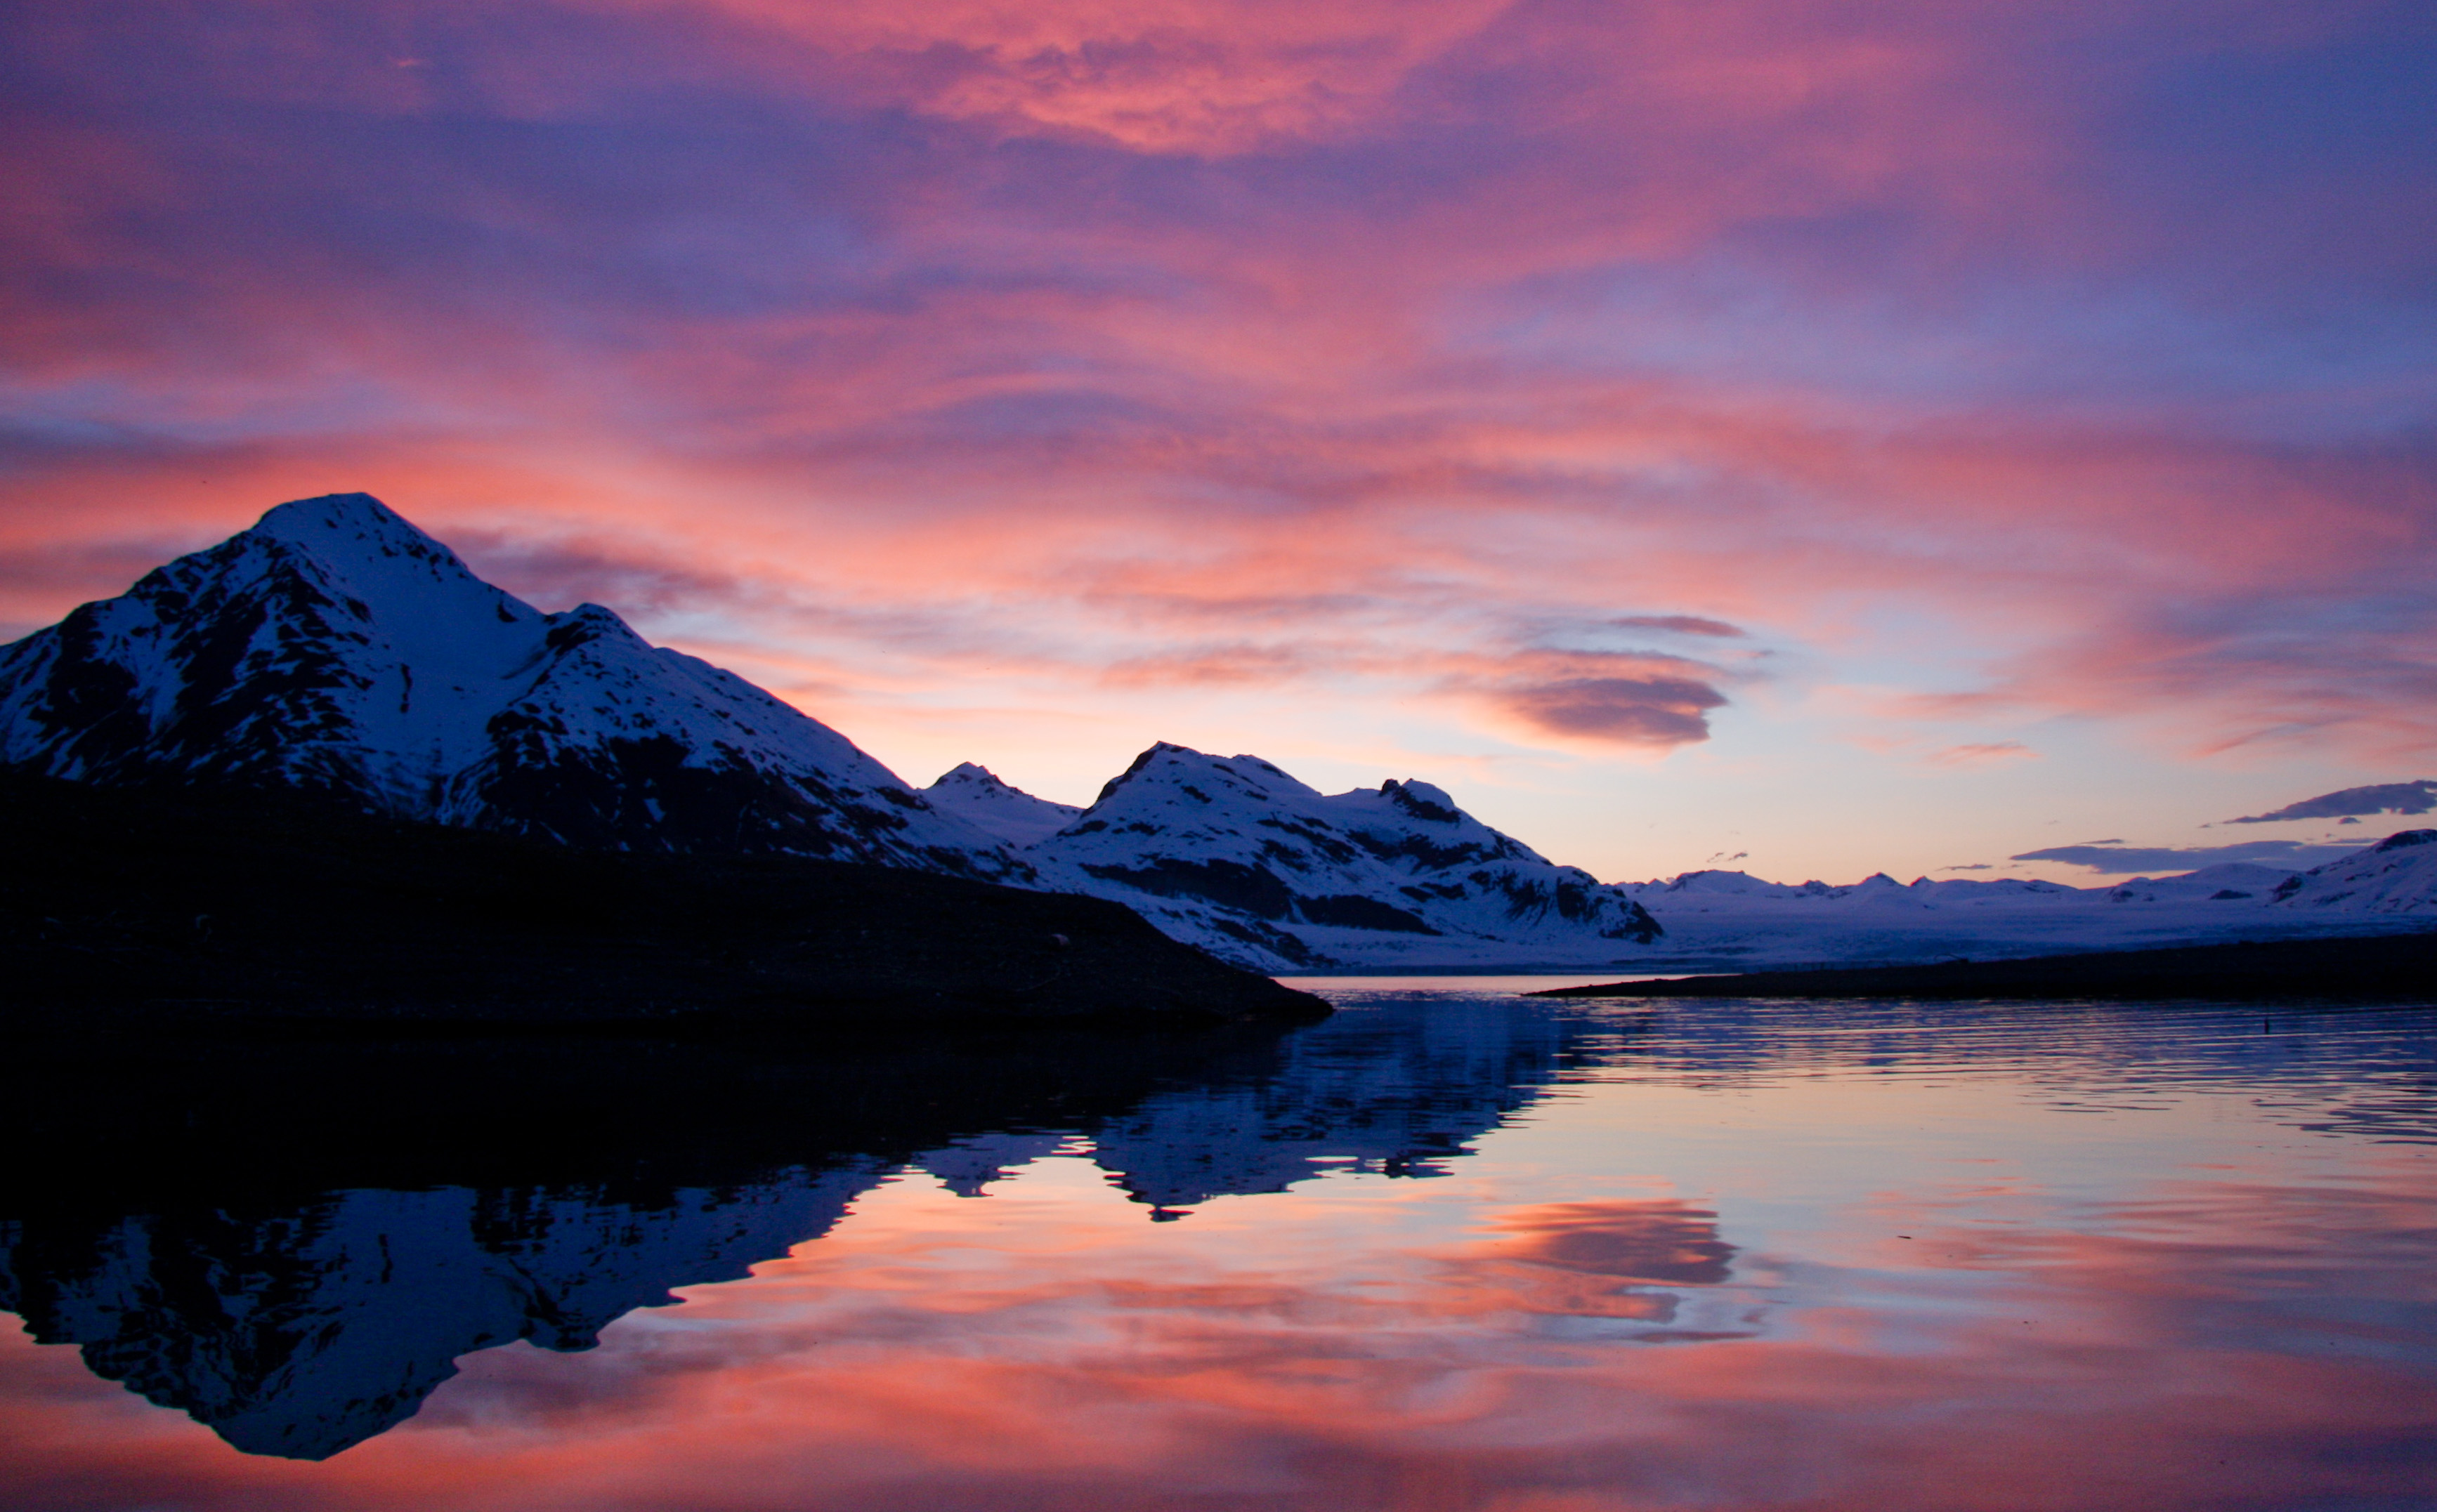
\includegraphics[height=
\paperheight,width=\paperwidth]{figures/yakutat_sunset}};}
} 


\begin{frame}[plain] % not in the handout
  \begin{columns}
    \column[C]{7.5cm}
  \begin{transbox}
    ``The tradition of glacier studies that we inherit draws upon two great legacies of the eighteenth and nineteenth centuries: classical physics and romatic enthusiasm for Nature.\\[.25em]
\ldots It is easy to undervalue the romantic contribution, but in glaciology, it would be a mistake to do so'' \\[.5em]
\emph{Garry Clark, J. Glaciol., 1987)}
  \end{transbox}
\end{columns}
\end{frame}


\setbeamertemplate{background canvas}
{
%
} 


\begin{frame}
  \frametitle{Course Material}
 \begin{itemize}
    \item lecture is based on lectures by Ed Waddington \& Martin Truffer
    \item Martin's ``Continuum Mechanics'' script
    \item book recommendation: \cite{GreveBlatter_disg}
 \end{itemize}
  \def\newblock{}
  \bibliography{cryo}
\end{frame}



\lecture{Introduction to glacier flow}{Part I}

\section{Measurements \& Observations}
 
\begin{frame}
  \frametitle{How does a glacier move?}
  \centering{
    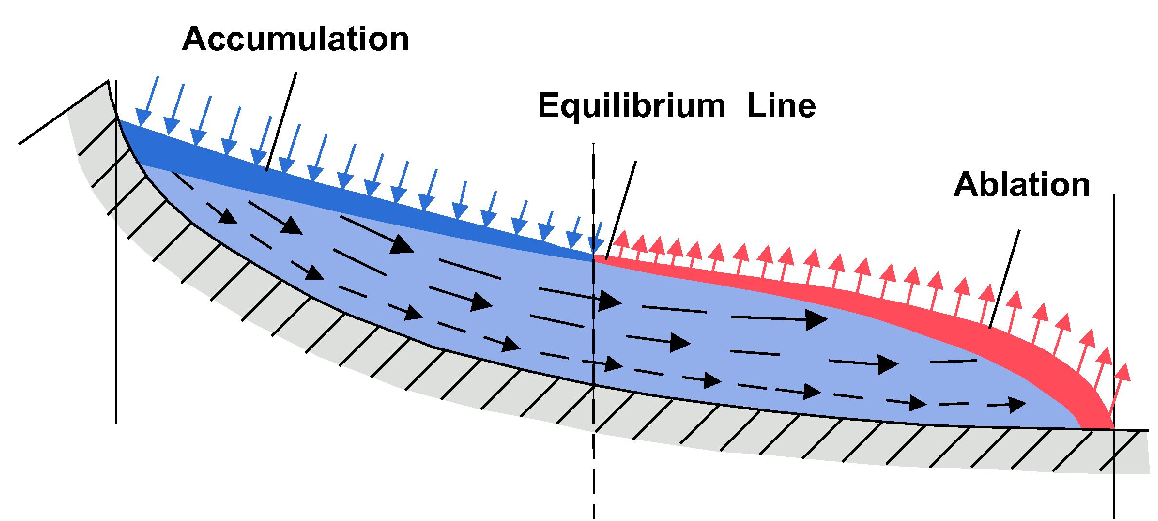
\includegraphics[width=.65\textwidth]{figures/flow_acc_abl}
  }
  \begin{block}{In a nut shell:}
    \begin{itemize}
    \item The ice can deform as a viscous fluid
    \item The ice can slide over its substrate
    \item Well-described by continuum mechanics
    \end{itemize}
  \end{block}
\end{frame}


\begin{frame}
  \frametitle{Measurements \& Observations}
    \begin{block}{1779 Gravitation theory by de~Saussure}
      H.~B. de~Saussure observes sliding
      \begin{itemize}
        \item ``\ldots the weight of the ice might be sufficient to urge it down the slope of the valley, if the sliding motion were aided by the water flowing at the bottom.''
      \end{itemize}
    \end{block}
    \begin{block}{1827-1836 Hugi Block}
      J.~Hugi observed that a boulder moved $1315\,\text{m}$ downstream between 1827 and 1836
      \begin{itemize}
        \item we would interpret this as clear evidence of glacier flow
        \item but back then, some people argued that a boulder slides on the glacier surface, the glacier itself is motionless
      \end{itemize}
    \end{block}
\end{frame}

\begin{frame}
  \frametitle{Measurements \& Observations}
  \begin{figure}
    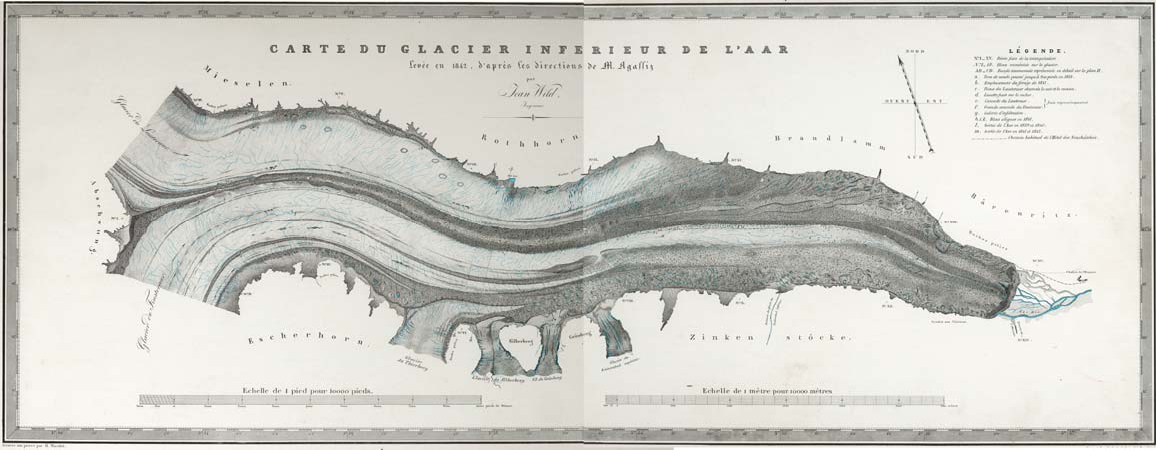
\includegraphics[width=8cm]{figures/agassi}%
  \end{figure}
    \begin{block}{1840-1846 Dilatation theory by L. Agassiz}
      \begin{itemize}
        \item glacier ice contains innumerable fissures and capillary tubes
        \item during the day, these tubes absorb the water
        \item and during the night, the water freezes
        \item this distension exerts a force and propels the glacier in the direction of least resistance
      \end{itemize}
    \end{block}
\end{frame}



\begin{frame}
  \frametitle{Measurements \& Observations}
  \begin{columns}
    \column[C]{4.25cm}
    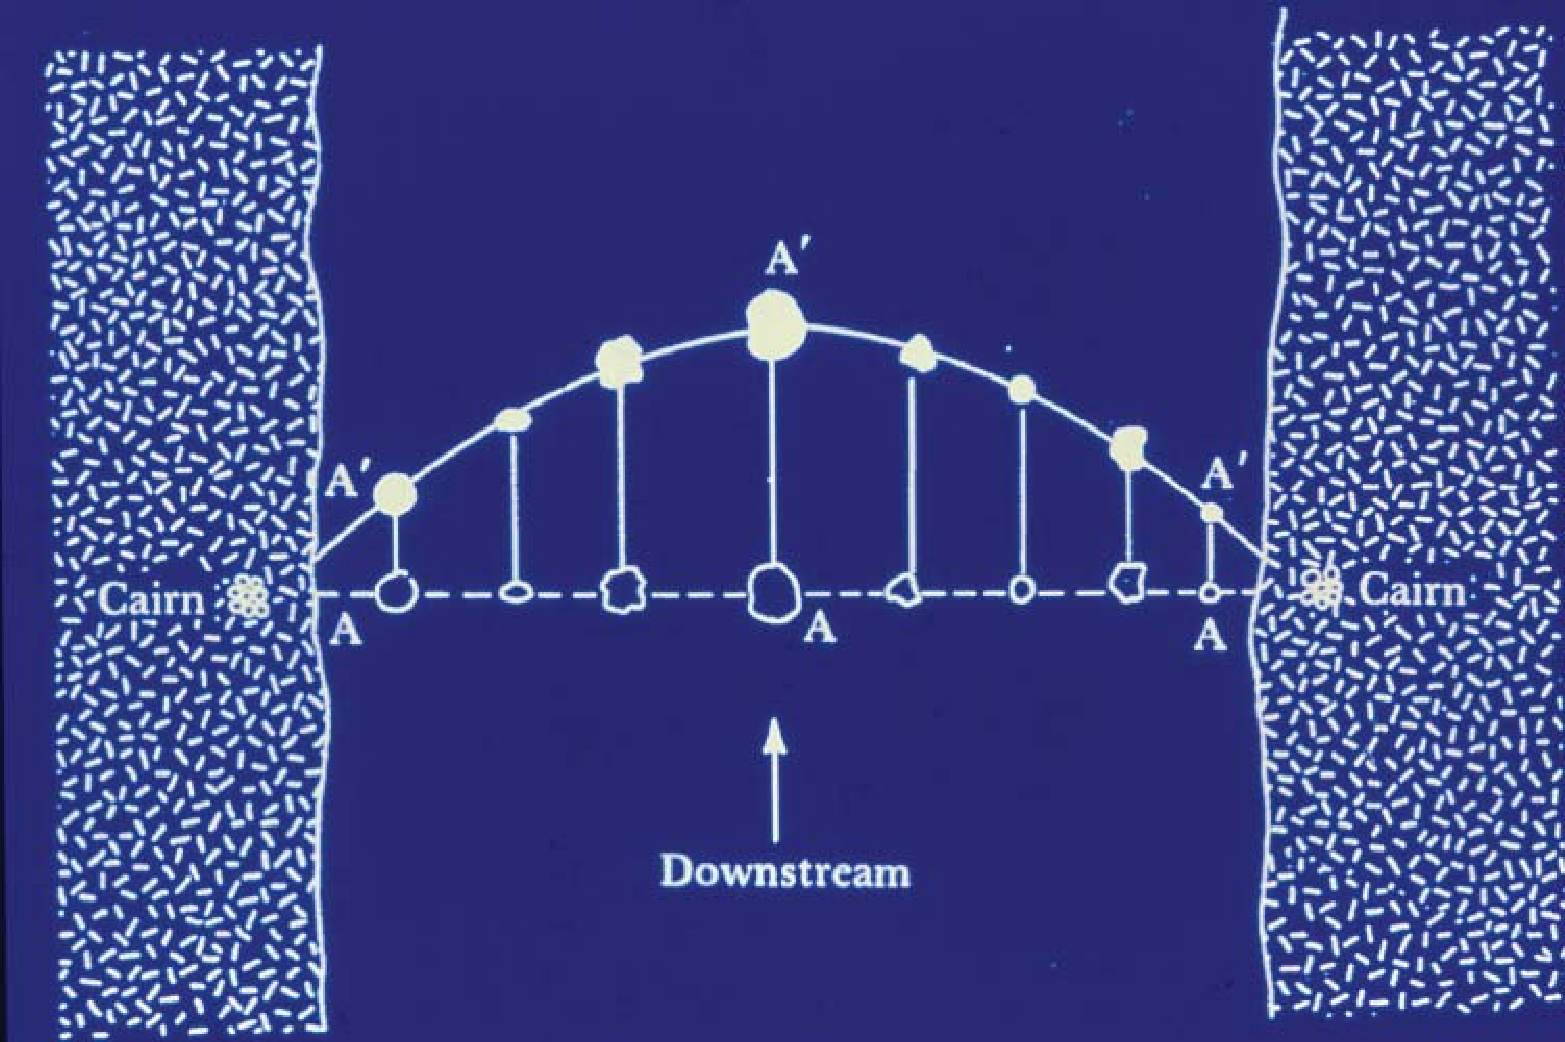
\includegraphics[width=4cm]{figures/geschw_prof_oberfl}%
    \vskip1em
    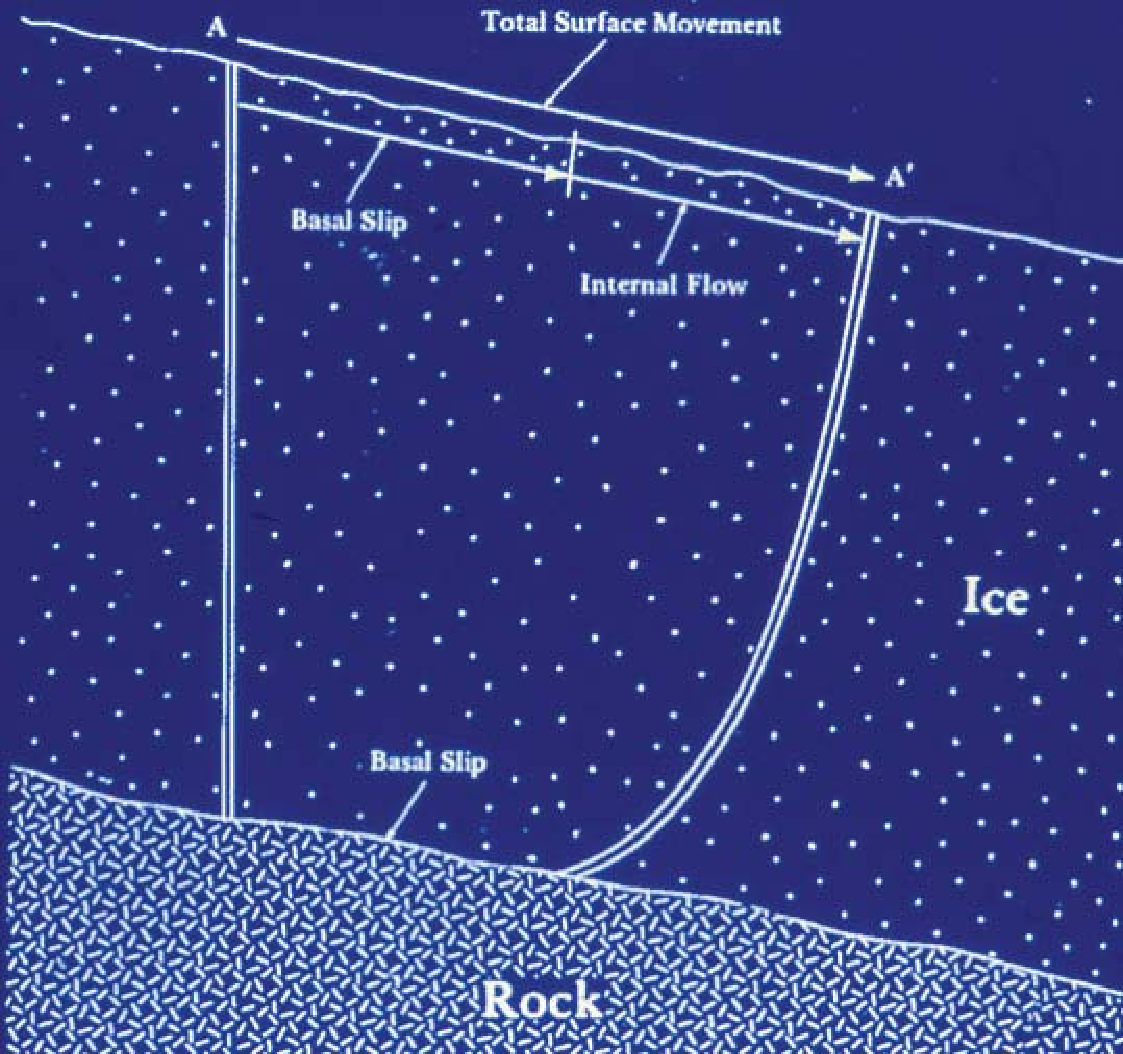
\includegraphics[width=4cm]{figures/geschw_vert_prof}%
    \column[C]{7.75cm}
    \begin{block}{1864-1930 Viscous flow theory by J.~Forbes}
      \begin{itemize}
      \item made his own observations on Mer de Glace, France
      \item glacier flows fastest in the center
      \item opposes Agassi's theory
      \item if the dilatation theory were true
      \item then flow would be greatest at sunset
      \item and near the glacier margins
      \end{itemize}
    \end{block}
  \end{columns}
\end{frame}


\begin{frame}
  \frametitle{Measuring surface velocities}
  \begin{columns}
    \column[C]{4.5cm}
    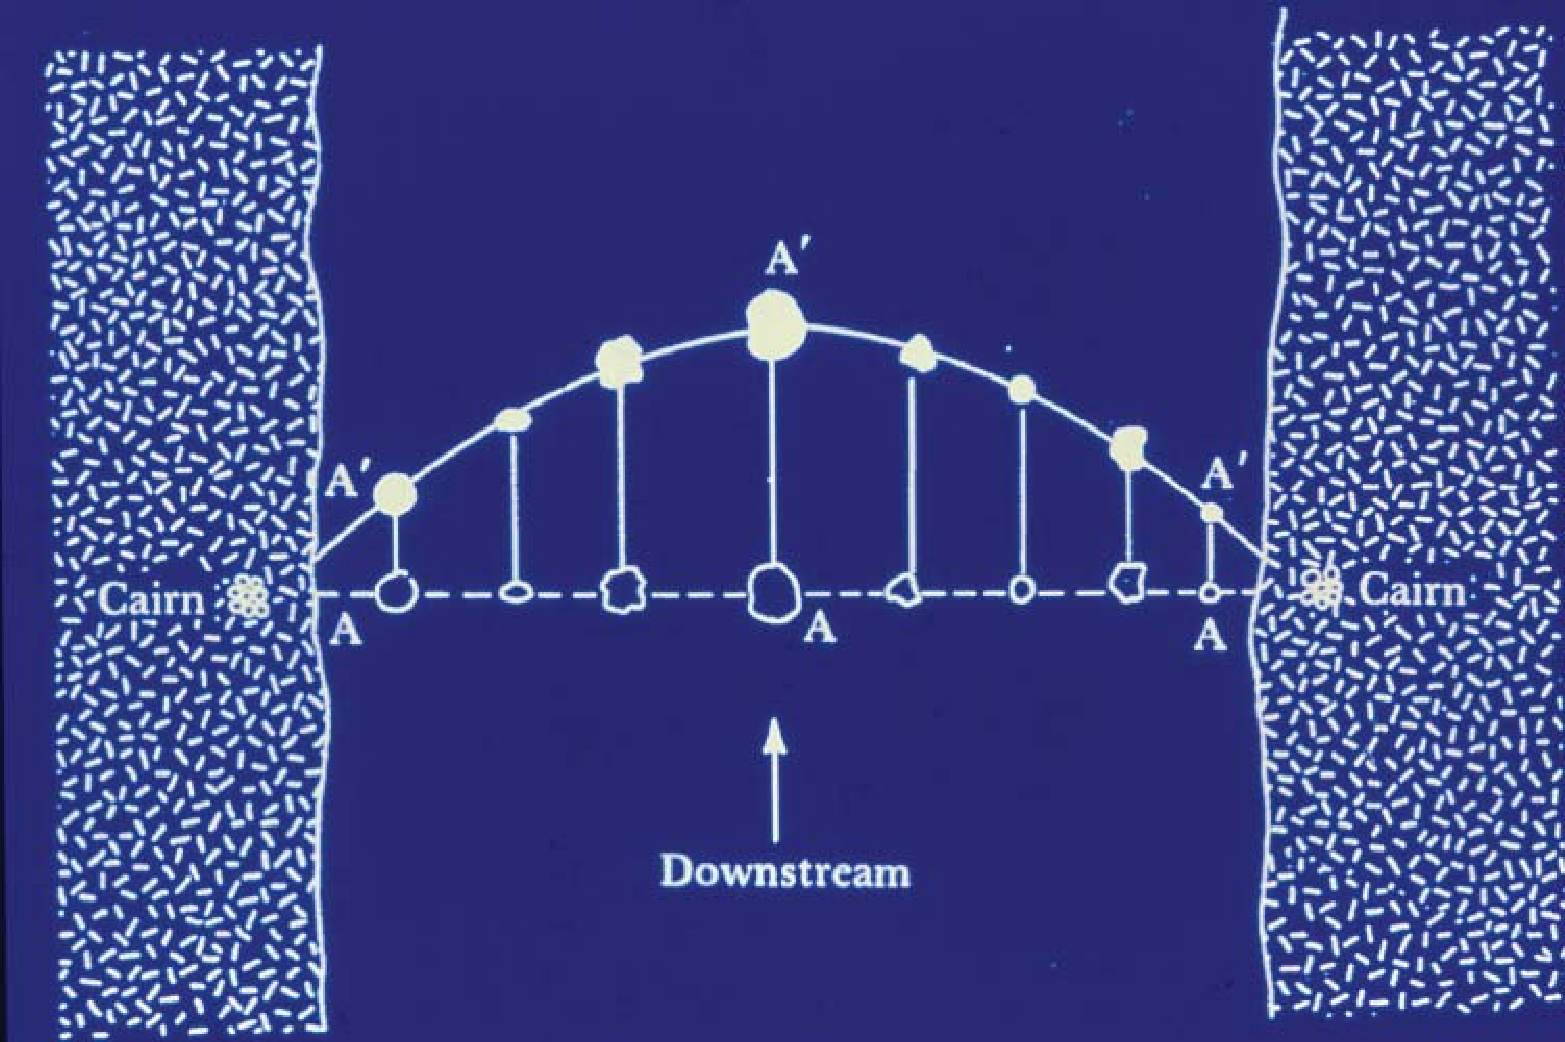
\includegraphics[width=4.5cm,angle=270]{figures/geschw_prof_oberfl}%
   \column[C]{7.5cm}
     \begin{itemize}
      \item Measuring angles (with Theodolite) and distances (with Electronic Distance Meter or EDM) from fixed stations on the glacier margins
        \item GPS (global positioning system)
        \item feature tracking in repeated aerial photography or satellite images
     \end{itemize}
 \end{columns}
\end{frame}


\begin{frame}
  \frametitle{Measuring surface velocities}
  \vspace{-2em}
  \begin{columns}
    \column[C]{5.5cm}
    \begin{figure}
    \includegraphics<1>[width=5.5cm]{figures/insar}%
    \includegraphics<2>[width=5.5cm]{figures/Joughin2010Fig6a}%
    \\ \small{credit: USGS, Joughin et al., 2010}
  \end{figure}
   \column[C]{6.5cm}
    \begin{block}{interferometric synthetic aperture radar (InSAR)}
      \begin{itemize}
      \item count fringes from a stationary point on bedrock
     \end{itemize}
    \end{block}
  \end{columns}
\end{frame}


\begin{frame}
  \frametitle{Measuring borehole tilt}
  \begin{columns}
    \column[C]{6.5cm}
    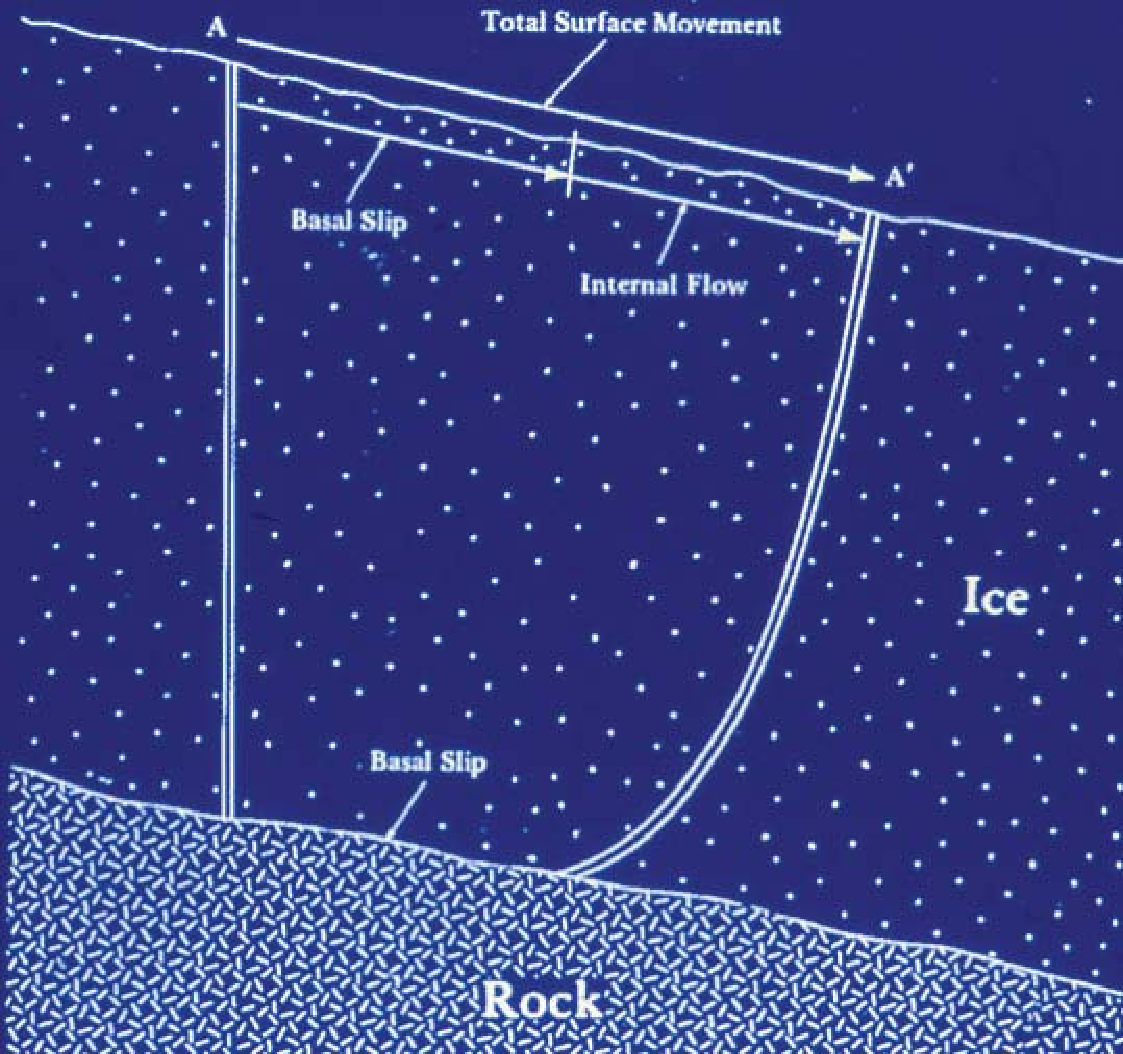
\includegraphics[width=6cm]{figures/geschw_vert_prof}%
   \column[C]{4.5cm}
     \begin{itemize}
      \item with tiltmeter (inclinometer)
     \end{itemize}
 \end{columns}
\end{frame}

\begin{frame}{Kinematic vs. Dynamics}
  \begin{block}{Kinematic description of flow}
    In a steady state,
    \begin{itemize}
    \item Flow required to transport away upstream accumulation
    \item Glacier has to adjust its shape to make this flow happen
    \item[$\Rightarrow$] Rheological properties don't figure in kinematic description
    \end{itemize}
  \end{block}
  \begin{block}{Dynamic description of flow}
    \begin{itemize}
    \item ice is a material with certain rheological properties (e.g. viscosity)
    \item Flow is determined by stresses applied to it
    \item[$\Rightarrow$] Accumulation/ablation don't figure in dynamic description
    \end{itemize}
  \end{block}
\end{frame}

\begin{frame}{``Glacier Flow'' Chart}
  \begin{figure}
    \centering{
      \tikzstyle{block} = [rectangle, draw, fill=light blue, 
    text width=5em, text centered]
\tikzstyle{today} = [rectangle, draw, fill=uaf blue, 
    text width=5em, text centered, rounded corners]
\tikzstyle{cloud} = [draw, ellipse,fill=light yellow,
    minimum height=2em]
\tikzstyle{line} = [draw, -latex']
    
\begin{tikzpicture}[node distance = 1.5cm, auto]
    % Place nodes
    \node [block] (climate) {climate};
    \node [cloud, below of=climate] (meteo) {meteorological process};
    \node [block, below of=meteo] (mass balance) {mass balance};
    \node [cloud, below of=mass balance] (dynamics) {ice dynamics processes};
    \node [today, left of=dynamics, node distance=5cm] (today) {this lecture};
    \node [block, below of=dynamics] (geometry) {glacier geometry};
    \node [right of=dynamics,node distance=5cm] (dummy) {};
    % Draw edges
    \path [line] (climate) -- (meteo);
    \path [line] (meteo) -- (mass balance);
    \path [line] (mass balance) -- (dynamics);
    \path [line] (dynamics) -- (geometry);
    \path [line] (today) -- (dynamics);
    \path [line] (geometry) -| (dummy);
    \path [line] (dummy) |- (mass balance);
    \path [line,dashed] (dummy) |- (climate);
  \end{tikzpicture}

    }
  \end{figure}
\end{frame}


\begin{frame}{Why is it so hard to predict the future of an ice sheet?}
  \begin{block}{It's easy because}
   \begin{itemize}
    \item composed of a single, largely homogenous material
    \item viscous flow is governed by the Navier-Stokes equations (19th century physics)
    \item move very slowly (turbulence, Coriolis force, and other inertial effects can be ignored)
   \end{itemize}
  \end{block}
  \begin{block}{It's so hard because}
   \begin{itemize}
    \item the stress resisting ice flow at the base can vary by orders of magnitude
    \item ocean interactions could trigger instabilities
  \end{itemize}
  \end{block}
\end{frame}


\section{Forces, Stress \& Strain}

\begin{frame}{Forces}
  \begin{itemize}
  \item a force is any influence that causes an object to undergo a change in speed, a change in direction, or a change in shape
  \item forces exist inside continuous bodies such as a glacier
  \item these forces can cause a glacier to deform
  \end{itemize}
\end{frame}

\begin{frame}{What is stress?}
  ``Stress'' is the force per unit area acting on a material
  \begin{displaymath}
    \sigma = \frac{F}{A}
  \end{displaymath}
  Inside a glacier, stresses are due to
  \begin{itemize}
  \item weight of the overlying ice (overburden pressure)
  \item shape of the glacier surface (pressure gradients)
  \end{itemize}
\end{frame}


\begin{frame}{Types of stress}
  As a force per unit area, stress has a direction
  \begin{columns}
    \column[c]{5cm}
    \begin{figure}
      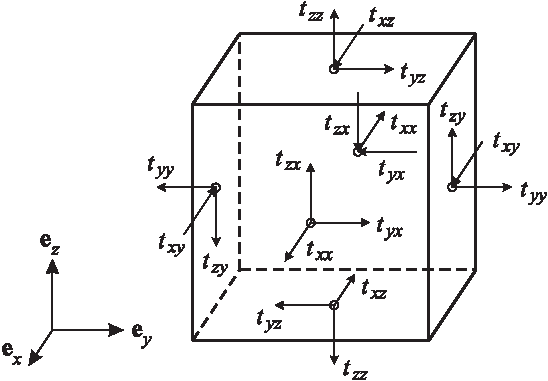
\includegraphics[width=4.75cm]{figures/fig_3_08}
    \end{figure}
    \column[c]{6.5cm}
   \begin{block}{}
      Force can be directed normal to the area
      \begin{itemize}
      \item Result is \alert{pressure} if the force is the same on all faces of a cube.
      \item Result is \alert{normal stress} if forces are different on different faces
      \end{itemize}
    \end{block}
    \begin{block}{} 
      Force can be directed parallel to the area
      \begin{itemize}
      \item Result is \alert{shear stress}
      \end{itemize}
    \end{block}
  \end{columns}
\end{frame}


\begin{frame}{Magnitudes of stress \& forces}
  Again, stress is force / (unit area)
     \begin{itemize}
      \item frictionless table
      \item water bottle in free fall
      \item stretching a rubber band
      \end{itemize}
\end{frame}

\begin{frame}{Pressure in a glacier}
  mass $m = \rho V$
     \begin{itemize}
      \item $\rho$ = ice density $\approx$ 900\,kg\,m$^{-3}$
      \item$V$ = Volume = Area $\times$ depth = $A \cdot z$
     \end{itemize}
     So pressure $p$ at depth $z$ is
     \begin{displaymath}
       p = \frac{m \cdot g}{A} = \frac{\rho \cdot A \cdot z \cdot g}{A} = \rho g z
     \end{displaymath}
     How deep do we have to drill into a glacier before the ice pressure is 1 atmosphere?
\end{frame}


\begin{frame}{Depth for 1\,atm pressure?}
    \begin{displaymath}
       z = \frac{p}{\rho\cdot g} = ?
     \end{displaymath}
     \begin{itemize}
     \item  So pressure rises by 1\,atm for every \alert{$x$}\,meters of depth in a glacier
     \item Does ice deform in response to this pressure?
     \end{itemize}
\end{frame}


\begin{frame}{Shear stress $\tau$}
  Total stress $t$ from ice column:
    \begin{displaymath}
       t = \rho V g = \rho\,g\,h
     \end{displaymath}
     \begin{itemize}
     \item How much of this weight will contribute to shear deformation?
     \item shear stress $\tau = \rho\,g\,h\,\sin{\alpha}$
     \item normal stress $\sigma = \rho\,g\,h\,\cos{\alpha}$
    \end{itemize}
\end{frame}


\begin{frame}{Shear stress in a glacier}
  \begin{itemize}
  \item $h$ = 130\,m
  \item $\alpha$ = 5$^{\circ}$
  \end{itemize}
  \begin{displaymath}
    \tau = \rho\,g\,h\,\sin{\alpha}
  \end{displaymath}
  \begin{beamercolorbox}[rounded=true,shadow=true]{boxed}
    Shear stress at the glacier base, $\tau_{b}$, is $\approx$ 1\,bar, which is a typical value for basal shear stress under a glacier
  \end{beamercolorbox}
\end{frame}
   

\begin{frame}{Are glacier thickness and slope related?}
  Suppose a glacier becomes thicker or steeper due to mass imbalance:
  \begin{itemize}
    \item it flows faster
    \item it quickly reduces thickness $h$ or slope $\alpha$, until $\tau_{b} \approx$ 1\,bar again
  \end{itemize}
  Can we then estimate glacier thickness ($z=h$) from its slope if we know $\tau_{b} \approx$ 1\,bar?
  \begin{displaymath}
    \tau = \rho\,g\,z\,\sin{\alpha} \quad \Rightarrow \quad h \sim \frac{\tau_{b}}{\rho\,g\,\sin{\alpha}}
  \end{displaymath}
   \begin{beamercolorbox}[rounded=true,shadow=true]{boxed}
      \begin{itemize}
       \item How are shear stress and shear strain rate (velocity) related?
       \end{itemize}
  \end{beamercolorbox}
\end{frame}


\begin{frame}{Strain rate $\dot\gamma$}
  \begin{figure}
  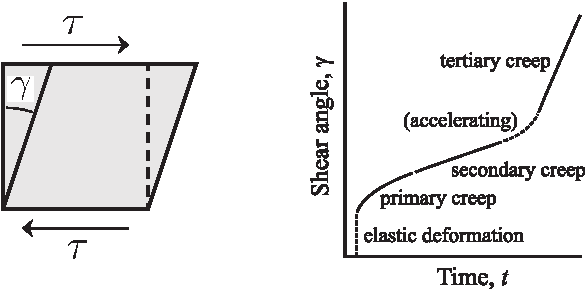
\includegraphics[width=7cm]{figures/fig_4_04}
  \end{figure}
  \begin{itemize}
  \item shear strain $\gamma = \frac{1}{2}\left( \frac{\Delta x}{\Delta z}\right) = \frac{1}{2} \gamma$
  \item shear strain rate $\dot \gamma = 1/2\,\left( \frac{\Delta x / \Delta z}{\Delta t}\right) = 1/2\,\left( \frac{\Delta u}{\Delta z}\right)$
  \end{itemize}
\end{frame}

\section{Material Science}

\begin{frame}
  \frametitle{Material Science}
  \begin{block}{Rheology}
    \begin{itemize}
    \item is the study of the flow of complex liquids or the deformation of soft solids.
    \item different materials respond differently to applied stresses
    \item We are not going through this in great detail.
    \item[$\Rightarrow$] For further information, consult the handout or
      \item take Martin Truffers ``Ice Physics 614''  class
    \end{itemize}
  \end{block}
  \begin{block}{We need to define}
    \begin{itemize}
   \item a relationship between shear stress and shear strain rate, $\tau = f(\dot \gamma)$
   \end{itemize}
  \end{block}
\end{frame}


\begin{frame}
  \frametitle{Example: Shear Experiment}
  \begin{itemize}
    \item apply constant shear stress $\boldsymbol{\tau}$
\end{itemize}
  \begin{columns}
    \column[c]{8cm}
    \begin{figure}
      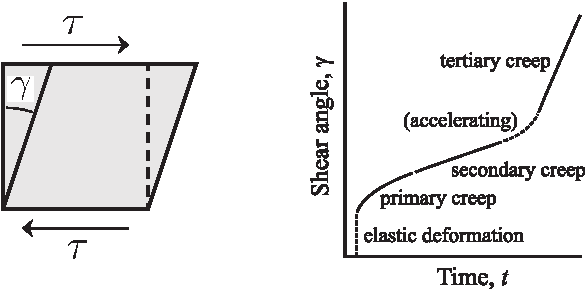
\includegraphics[width=6cm]{figures/fig_4_04}
    \end{figure}
    \column[c]{5cm}
    $\tau$ is the applied shear stress\\
    $\gamma$ is the shear angle\\
    $\dot\gamma$ is the shear rate
  \end{columns}
  \begin{itemize}
    \item initial elastic deformation
    \item primary creep: shear rate $\dot\gamma$ decreases with time
    \item \alert{secondary creep}: shear rate remains constant
    \item acceleration phase
    \item tertiary creep: constant shear rate (but higher) 
 \end{itemize}
\end{frame}


\begin{frame}
  \frametitle{Example: Shear Experiment}
  \begin{columns}
    \column[c]{8cm}
    \begin{figure}
      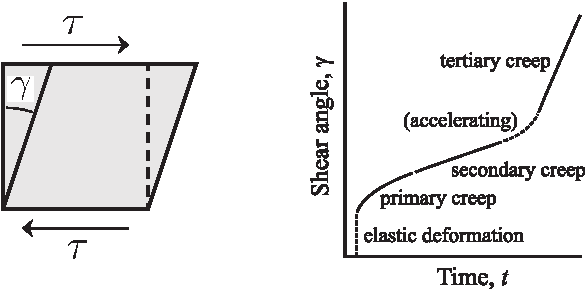
\includegraphics[width=6cm]{figures/fig_4_04}
    \end{figure}
    \column[c]{5cm}
    $\tau$ is the applied shear stress\\
    $\gamma$ is the shear angle\\
    $\dot\gamma$ is the shear rate
  \end{columns}
  \vskip1em
  This suggests that
  \begin{itemize}
  \item the shear rate is a function of the applied shear stress, temperature $T$, and pressure $p$
    \begin{equation*}
      \dot\gamma = \dot\gamma\left(\tau,T,p\right)
    \end{equation*}
   \end{itemize}
 \end{frame}


\begin{frame}
  \frametitle{Example: Shear Experiment}
  \begin{columns}
    \column[c]{8cm}
    \begin{figure}
      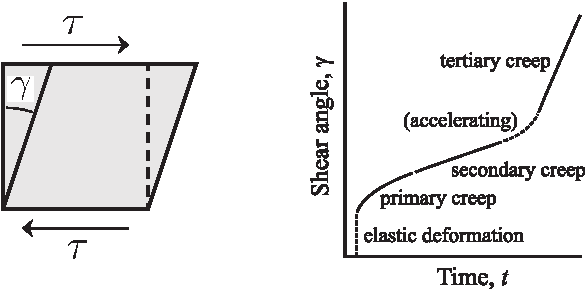
\includegraphics[width=6cm]{figures/fig_4_04}
    \end{figure}
    \column[c]{5cm}
    $\tau$ is the applied shear stress\\
    $\gamma$ is the shear angle\\
    $\dot\gamma$ is the shear rate
  \end{columns}
  \vskip1em
  \begin{itemize}
  \item The dynamic viscosity $\eta$ relates shear stress and shear rate
    \begin{equation*}
      \tau = \eta\left(T,p,\vert \dot\gamma \vert\right)\dot\gamma
    \end{equation*}
  \end{itemize}
\end{frame}


\begin{frame}
  \frametitle{Constitutive behavior of ice}
  \begin{displaymath}
    \dot \gamma = 2\,A(T,p)\,\tau^{n-1}\tau
  \end{displaymath}
  \\
  \begin{equation*}
    \begin{array}{rcll}
      A(T,p) & = & A_{0} e^{-Q/(RT)} &\qquad \text{Arrhenius law}
    \end{array}
  \end{equation*}
  \begin{itemize}
  \item $A$ is called \alert{rate factor} (ice softness)
  \item $Q$ and $R$ are the activation energy and the gas constant, respectively
  \item $n$ is the exponent of the flow law, usually taken as $n=3$
  \end{itemize}
  \vskip1em
  This is known as \alert{Glen's flow law} or \alert{Glen-Steinemann flow law} but similar to Norton's flow law for the flow of steel at high temperatures
\end{frame}

\begin{frame}
  \frametitle{Temperature dependence}
  With some emperically-derived values for Q we get:
    \begin{figure}
      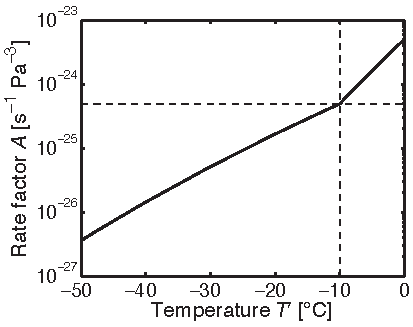
\includegraphics[width=6cm]{figures/fig_4_05}
    \end{figure}
    \begin{itemize}
      \item ice at 0\,$^{\circ}$C is about 1000$\times$ softer than ice at -50\,$^{\circ}$C
    \end{itemize}
\end{frame}

\begin{frame}{Thin-film flow}
  \begin{figure}
    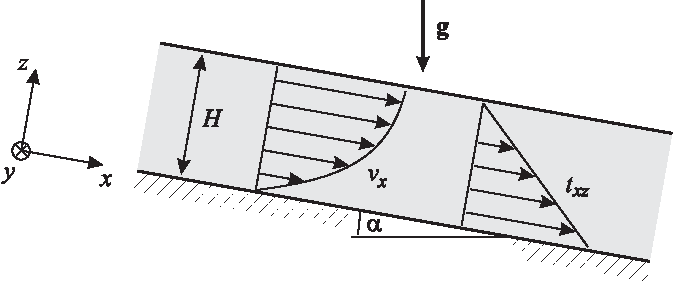
\includegraphics[width=7cm]{figures/fig_3_11}
  \end{figure}
  \begin{equation*}
    \begin{array}{ccl}
      \frac{\partial u}{\partial z}  & = &  2\,A(T,p)\,\tau^{n-1}\tau \qquad \Rightarrow \\[1em]
      u_{h} - u_{b} &  = & \int_{0}^{h} 2\,A\left(\rho\,g\,\sin{\alpha}\right)^{n}\,dz =
    \end{array}
  \end{equation*}
  \\[.75em]
  We assume $u_b=0$, i.e. glacier is frozen to the bed
\end{frame}


\begin{frame}{Basal sliding}
  Despite decades of intensive research, basal sliding remains one of the grand unsolved problems. We know:
  \begin{itemize}
  \item sliding is a function of basal water pressure and bed roughness
  \item if ice is underlain by till, experiments suggest a plastic or nearly-plastic behavior
  \end{itemize}
  \vspace{1em}
  \begin{columns}
    \column[C]{7.5cm}
    \begin{beamercolorbox}[rounded=true,shadow=true]{boxed}
      Beyond the scope of this lecture
    \end{beamercolorbox}
  \end{columns}
\end{frame}

\frame[label=recap]{
\frametitle{Recap}
  \begin{itemize}
    \item so far, we have only considered shear stresses 
    \item while they are often the \emph{most} important ones in glacier flow,
    \item there are other stresses (e.g. normal stresses) which can be important too
    \item we have assumed ice surface and bed surface are parallel
    \item let's step back and look at the bigger picture
    \item yep, we will need basic calculus and some continuum mechanics
  \end{itemize}
}


\lecture{Field equations for ice flow}{Part II}

\againframe{recap}

\begin{frame}{Continuum Mechanics}
Continuum mechanics is the application of \alert{classical mechanics} to \alert{continuous media}. So
\vspace{1em}
\begin{itemize}
\item What is classical mechanics?
\item What are continous media
\end{itemize}
\end{frame}


\begin{frame}{Classical Mechanics}
In classical mechanics, we deal with two type of equations
\vspace{1em}
\begin{itemize}
\item conservation (balance) equations (fundamental to physics)
\item material equations (less fundamental)
\end{itemize}
 \begin{block}{Balance Laws}
    \begin{itemize}
    \item balance of mass
    \item balance of linear momentum
    \item balance of angular momentum
    \item balance of energy
    \end{itemize}
  \end{block}
  \begin{block}{Material Laws / Constitutive Equations / Closures}
    \begin{itemize}
      \item often obtained from experiments and theoretical considerations (such as material objectivity)
   \end{itemize}
  \end{block}
\end{frame}


\begin{frame}{Classical Mechanics}
  \begin{block}{Densities}
    \begin{itemize}
    \item classical mechnics has concept of point mass
    \item determine velocity (and acceleration) by looking at changes (and rate of changes) in position $\Rightarrow$ \alert{Kinematics}
    \item how do forces affect a mass? $\Rightarrow$ \alert{Dynamics}
\end{itemize}
\end{block}
\vspace{1em}
Volume $\Omega$ has mass $m$, then 
\vspace{1em}
    \begin{equation}
      \begin{array}{lccll}
        \textsf{mass} \quad & m &=& \int_{\Omega} \rho\,dv, & \, \rho \quad \textsf{mass density}\\[.25em]
        \textsf{linear momentum} \quad& mv &=& \int_{\Omega} \rho v\,dv, & \, \rho v\quad \textsf{linear momentum density} \\[.25em]
        \textsf{internal energy} \quad & U &=& \int_{\Omega} \rho u\,dv, & \, \rho u\quad \textsf{energy density}
      \end{array}
    \end{equation}
  \end{frame}


\begin{frame}
  \frametitle{General Balance Laws}
  Imagine a volume $\Omega$ enclosed by a boundary $\partial \Omega$
   \begin{eqnarray}
      G(t) &=& \int_{\Omega} g(x,t)\,d v \\
      S(t) &=& \int_{\Omega} s(x,t)\,d v
    \end{eqnarray}
    \begin{columns}
      \column[C]{0.1cm}
      $G,g$ \\
      $S,s$ \\
     \column[C]{6cm}
      physical quantity and density\\
      supply and density \\
   \end{columns}
\end{frame}


\begin{frame}
  \frametitle{General Balance Laws}
  $G$ can only change if
 \begin{itemize}
   \item if there is a supply $S$ within $\Omega$
   \item if there is a flux $F$ of $G$ through the boundary $\partial \Omega$
  \end{itemize}
  \begin{equation}
   F(t) = \oint_{\partial \Omega} \left(g\mathbf{v} + \phi(x,t)\right) \cdot \mathbf{n}\,da
   \end{equation}
    \begin{columns}
      \column[C]{0.1cm}
      $g\mathbf{v}$ \\
      $\phi(x,t)$ \\
     \column[C]{7cm}
      transport of $g$ with velocity $\mathbf{v}$ through $\partial \Omega$\\
      flux density (defined later) \\
   \end{columns}
\end{frame}


\begin{frame}
  \frametitle{General Balance Laws}
  \begin{itemize}
 \item General balance law is:
  \end{itemize}
  \begin{eqnarray}
    \frac{dG}{dt} &=& S - F \\[1em]
    \frac{d}{dt} \int_{\Omega} g(t)\,dv &=& \int_{\Omega} s(x,t)\,d v - \oint_{\partial \Omega} \left(g\mathbf{v} + \phi\right) \cdot \mathbf{n}\,da
  \end{eqnarray}
\end{frame}

\begin{frame}
  \frametitle{General Balance Laws}
  \begin{itemize}
  \item Assume that $G \ne G(t)$ thus integral and differential can be exchanged
  \item Use Gauss' Theorem:
    \begin{displaymath}
      \oint_{\partial \Omega} \left(g\mathbf{v} + \phi\right) \cdot \mathbf{n}\,da = \int_{\Omega} \nabla \cdot \left(g\mathbf{v} + \phi\right)\,dv
   \end{displaymath}
  \item We can then write
  \end{itemize}
  \begin{eqnarray}
   \int_{\Omega} \frac{\partial g}{\partial t}\,dv &=& \int_{\Omega} s(x,t)\,d v - \int_{\Omega} \nabla \cdot \left(g\mathbf{v} + \phi\right)\,dv
  \end{eqnarray}
\end{frame}

\begin{frame}
  \frametitle{General Balance Laws}
  \begin{itemize}
  \item We made no assumption about the shape and size of $\Omega$ 
  \item We can make $\Omega$ infinitely small
  \end{itemize}
  \begin{equation}
    \frac{\partial g}{\partial t} = s(t)- \nabla \cdot \left(g\mathbf{v} + \phi\right)
  \end{equation}
  or
  \begin{equation}
    \frac{d g}{d t} = \frac{\partial g}{\partial t} + \mathbf{v}\cdot \nabla g = s(t)- \nabla \cdot  \left(\mathbf{v} + \phi\right)
  \end{equation}
\end{frame}

\section{Mass Balance}

\begin{frame}
  \frametitle{Mass Balance}
  \begin{itemize}
    \item the mass of a material volume cannot change, $\text{d} M/\text{d} t=0$
    \end{itemize}
    \begin{columns}
      \column[C]{1cm}
      $g = \rho$ \\
      $\boldsymbol{\phi} =0 $ \\
     $s = 0$ \\
      \column[C]{6cm}
      mass density \\
      flux of $g$ through the boundary \\
     supply of $g$
    \end{columns}
    \vskip1em
    from the above we get
   \begin{equation}
      \frac{\partial \rho}{\partial t} + \nabla \cdot \left(\rho \mathbf{v}\right) = 0
    \end{equation}
    $\Rightarrow$ known as the \alert{continuity equation}\\
    We assume ice is \emph{incompressible} (density does not change), then
    \begin{equation}
      \nabla \cdot \mathbf{v} = 0
    \end{equation}
  \end{frame}


\section{Momentum Balance}

\begin{frame}
  \frametitle{Momentum Balance}
  Newton's Second Law
  \begin{itemize}
    \item total rate of change of momentum $\mathbf{P}$ equals sum of all forces $\mathbf{F}$
    \begin{equation}
      \frac{\text{d} \mathbf{P}}{\text{d} t} = \mathbf{F} = \underbrace{\oint_{\partial \omega} \mathbf{t}_{\mathbf{n}} \, \text{d} a}_{\text{internal}} +\underbrace{\int_{\omega} \mathbf{f} \, \text{d} v}_{\text{external}}
    \end{equation}
    \item $\mathbf{P}$ and $\mathbf{F}$ are vector quantities
    \item identify the internal stress vector $\mathbf{t}_{\mathbf{n}} = \mathbf{T}\mathbf{n}$, see p. 31
    \item $\mathbf{T}$ is the \alert{Cauchy stress tensor}
    \item external forces $\mathbf{f}$ are, e.g. gravity or the Coriolis force (forces are a source of momentum)
    \end{itemize}    
  \end{frame}


\begin{frame}
  \frametitle{The Cauchy Stress Tensor}
  We've already introduced shear stress, but forces can be applied on different faces and in different directions
  \begin{columns}
    \column[c]{6cm}
    \begin{figure}
      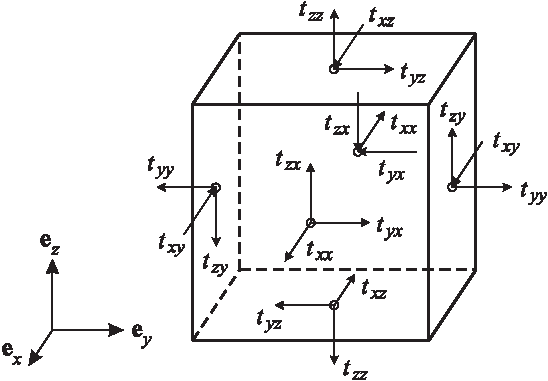
\includegraphics[width=5.cm]{figures/fig_3_08}
    \end{figure}
    \column[c]{5cm}
  \begin{displaymath} 
    \mathbf{T} = \left( 
      \begin{array}{ccc} 
        t_{xx} & t_{xy} & \alert{t_{xz}} \\ 
        t_{yx} & t_{yy} & t_{yz} \\ 
        t_{zx} & t_{zx} & t_{zz} 
      \end{array} 
    \right) 
  \end{displaymath}
  \begin{itemize}
  \item We identify $\tau = t_{xz}$
  \end{itemize}
\end{columns}
  \vskip1em
  For example
$    \mathbf{t}_{\mathbf{e}_{z}} =
    \left(
      \begin{array}{c}
        t_{xz}\\
        t_{yz}\\
        t_{zz}
      \end{array}
    \right)
 $ is the stress vector of a cut along the xy-plane
\end{frame}


\begin{frame}
  \frametitle{Momentum Balance}
  \begin{equation}
    \frac{\partial \left(\rho \mathbf{v}\right)}{\partial t}  = -\nabla \cdot \left(\rho \mathbf{v}\otimes\mathbf{v}\right) + \nabla \cdot \mathbf{T} + \mathbf{f}
  \end{equation}
  \begin{columns}
    \column[C]{2cm}
    $g = \rho \mathbf{v}$ \\
    $\boldsymbol{\phi} = - \mathbf{T} $ \\
    $s = \mathbf{f}$ \\
    \column[C]{6cm}
      momentum density \\
      flux of $g$ through the boundary \\
      supply of $g$
    \end{columns}
    By using the mass balance, we can write
    \begin{equation}
      \frac{\text{d}\left(\rho\mathbf{v}\right)}{\text{d} t} = \nabla \cdot \mathbf{T} + \mathbf{f}
    \end{equation}
   \begin{beamercolorbox}[rounded=true,shadow=true]{boxed}
     \begin{block}{What's new?}
       \begin{itemize}
       \item shear stress $\tau$ replaced with Cauchy stress tensor $\mathbf{T}$
       \end{itemize}
     \end{block}
   \end{beamercolorbox}
 \end{frame}
  

\begin{frame}
  \frametitle{Momentum Balance}
  For glacier ice, we assume
  \begin{itemize}
  \item ice is incompressible
  \item acceleration term $\frac{\text{d}\left(\rho\mathbf{v}\right)}{\text{d} t}$ can be neglected
  \item supply of momentum is through gravity only, $\mathbf{f} = \rho \mathbf{g}$
  \end{itemize}
  \vspace{1em}
  The momentum balance for glacier flow is
  \begin{equation}
    \nabla \cdot \mathbf{T} + \rho \mathbf{g} = 0
  \end{equation}
\end{frame}

\section{Angular Momentum Balance}

\begin{frame}
  \frametitle{Angular Momentum Balance}
  \begin{itemize}
  \item  no, I don't want to do the whole derivation here
  \item if you're interested (or bored), go through Equations~3.77\,--\,3.83  in \cite{GreveBlatter_disg}
  \item here, we just use the result
  \item the stress tensor $\mathbf{T}$ is \alert{symmetric}
  \end{itemize}
  \begin{equation}
    \mathbf{T} = \mathbf{T}^{T}
 \end{equation}
\end{frame}


\section{Energy Balance}

\begin{frame}
  \frametitle{Energy Balance}
  \begin{itemize}
  \item  only the total energy (sum of kinetic and inner energy) is a \alert{conserved} quantity
  \item balance of kinetic energy is \alert{not an independent statement} but a mere consequence of the momentum balance
  \item here, we formulate the balance of specific inner energy, $u$:
  \end{itemize}
  \begin{equation}
    \rho\frac{\text{d} u}{\text{d} t} = - \nabla \cdot \mathbf{q} + \text{tr}\left(\mathbf{T}\cdot\mathbf{D}\right) + \rho r
  \end{equation}
\vskip1em
 \begin{columns}
   \column[C]{3cm}
   $g = u$ \\
   $\boldsymbol{\phi} = \mathbf{q} $ \\
   $p = \text{tr}\left(\mathbf{T}\cdot\mathbf{D}\right) $ \\
   $s = \rho r$ \\
   $\mathbf{D} = 1/2\left(\mathbf{v}^{T}+\mathbf{v}\right)$
   \column[C]{6cm}
   specific internal energy \\
   heat flux \\
   dissipation power \\
   specific radiation power\\
   \alert{strain rate} or \alert{velocity gradient} tensor
 \end{columns}
\end{frame}



\begin{frame}
  \frametitle{Balance Equations}
  \begin{equation*}
  \begin{array}{lcclc}
    \text{mass} \quad &  \frac{\text{d} \rho}{\text{d} t} & = & -\rho\nabla \cdot \mathbf{v} \quad & (1)\\[.25em]
    \text{momentum} \quad & \rho \frac{\text{d} \mathbf{v}}{\text{d} t} & = & \nabla \cdot \mathbf{T} + \mathbf{f} \quad & (3) \\[.25em]
    \text{internal energy} \quad & \rho\frac{\text{d} u}{\text{d} t} & = & - \nabla \cdot \mathbf{q} + \text{tr} \left(\mathbf{T}\cdot\mathbf{D}\right) + \rho r\quad & (1)
  \end{array}
  \end{equation*}
\centering{
 \begin{columns}
   \column[T]{4cm} \centering{
   left-hand side \\
   $\rho$ (1)\\
   $\mathbf{v}$ (3)\\
   $u$ (1)
   }
   \column[T]{4cm} \centering{
   right-hand side \\
   $\mathbf{T}$ (6)\\
   $\mathbf{q}$ (3)
  }
 \end{columns}
  }
  \begin{itemize}
   \item so we have 5 equations for 14 unknown fields
   \item the system is highly under-determined
   \item[$\Rightarrow$] \alert{closure relations} required
 \end{itemize}
\end{frame}



\begin{frame}
  \frametitle{Closure Relations}
  \begin{itemize}
    \item \alert{balance equations} are universally valid
    \item \alert{closure relations} describe the specific behavior of a material
    \item \alert{closure relations} are often called \alert{constitutive equations}
  \end{itemize}
\end{frame}


\section{Constitutive Equations}


\begin{frame}
  \frametitle{Material Science}
  \begin{block}{Rheology}
    \begin{itemize}
    \item is the study of the flow of complex liquids or the deformation of soft solids.
    \item We are not going through this in great detail.
    \item[$\Rightarrow$] For further information, consult the handout or
      \item take Martin Truffers ``Ice Physics 614''  class
    \end{itemize}
  \end{block}
  \begin{block}{We need to define}
    \begin{itemize}
    \item a constitutive equation for the heat flux $\mathbf{q}$
    \item and for the internal energy $u$
    \item a relationship between stress and strain, $\mathbf{T} = f(\mathbf{D})$
   \end{itemize}
  \end{block}
\end{frame}


\begin{frame}
  \frametitle{Generalization}
  \begin{block}{Assume}
  \begin{itemize}
  \item secondary creep
  \item incompressibility of ice $\Rightarrow$ uniform pressure does not lead to deformation
    $\mathbf{T} = \underbrace{-p\mathbf{I}}_{\text{isotropic}} + \underbrace{\mathbf{T}'}_{\text{deviatoric}}$
\item with the pressure $p=-1/3\text{tr}{\mathbf{T}}$
  \end{itemize}
\end{block}
  \vskip.5em
  The only non-straightforward step from
  \begin{equation}
    \tau = \eta\left(T,p,\vert \dot\gamma \vert\right)\dot\gamma
  \end{equation}
  to
  \begin{equation}
    \mathbf{T}' = \eta\left(T,p,\vert \bullet \vert\right)\mathbf{D}
  \end{equation}
  is the generalization of $\vert \dot\gamma\vert$
\end{frame}

\begin{frame}
  \frametitle{Generalization}
  \begin{equation}
    \mathbf{T}' = \eta\left(T,p,\vert \bullet \vert\right)\mathbf{D}
  \end{equation}
  is a relation between two tensors (i.e. $\mathbf{T}$ and $\mathbf{D}$)
  \begin{itemize}
  \item \alert{material objectivity} tells us that such a relationship must be independent of the chosen vector basis
  \item a second rank tensor has 3 scalar invariants
    \begin{eqnarray}
      I_{\mathbf{T}'} & = & \text{tr}\mathbf{T}' \\
      II_{\mathbf{T}'} & = & 1/2\left(\left(\text{tr}\mathbf{T}'\right)^{2}  -\text{tr}\left(\mathbf{T}'\right)^{2}\right)\\
      III_{\mathbf{T}'} & = & \text{det}\,\mathbf{T}'
    \end{eqnarray}
    \item $\text{tr}\mathbf{T}'=0$ for incompressible media
    \item $\sigma_{\text{e}} = \sqrt{II_{\mathbf{T}'}}$ is the \alert{effective stress}
    \item role of $ III_{\mathbf{T}'}$ is not clear, but lab experiments indicate that the third invariant is not important
  \end{itemize}
\end{frame}

\begin{frame}
  \frametitle{Generalization}
  Numerous lab experiments and field measurements suggest
    \begin{equation}
      \frac{1}{\eta\left(T,p,\sigma_{\text{e}}\right)} =2A\left(T,p\right)f\left(\sigma_{\text{e}}\right)
    \end{equation}
    where
    \begin{equation*}
      \begin{array}{rcll}
      A(T,p) & = & A_{0} e^{-Q/(RT)} &\qquad \text{Arrhenius law}\\[.25em]
      f\left(\sigma_{\text{e}}\right) & = &\sigma_{\text{e}}^{n-1} &\qquad \text{power law}
      \end{array}
    \end{equation*}
\end{frame}


\begin{frame}
  \frametitle{Generalization}
   \begin{beamercolorbox}[rounded=true,shadow=true]{boxed}
     \begin{block}{What's new?}
       \vspace{1em}
       We have replaced
       \begin{equation}
         \dot \gamma = \eta\left(T,p,\vert \tau \vert\right)\tau
       \end{equation}
       by
       \begin{equation}
         \mathbf{D} = \eta\left(T,p,\vert \sigma_{\sf{eff}} \vert\right)\mathbf{T}'
       \end{equation}  
     \end{block}
   \end{beamercolorbox}
 \end{frame}


\begin{frame}
  \frametitle{Calorimetric Equation of State}
  Internal energy, $u$ depends linearly on temperature, $T$,
  \begin{equation}
    u = u_{0} + c\left(T-T_{0}\right)
  \end{equation}
  \begin{itemize}
  \item $u_{0}$ is a reference value at a reference temperature $T_{0}$
  \item $c$ is the heat capacity (a measure how much heat is needed to raise the temperature by a certain amount)
  \item we obtain
  \end{itemize}
  \begin{equation}
    \frac{\text{d} u}{\text{d} t} =     c \frac{\text{d} T}{\text{d} t} 
  \end{equation}
\end{frame}

\begin{frame}
  \frametitle{Heat Flux}
 \begin{block}{Fourier's law of heat conduction}
  \begin{columns}
    \column[c]{5.5cm}
  \begin{figure}
    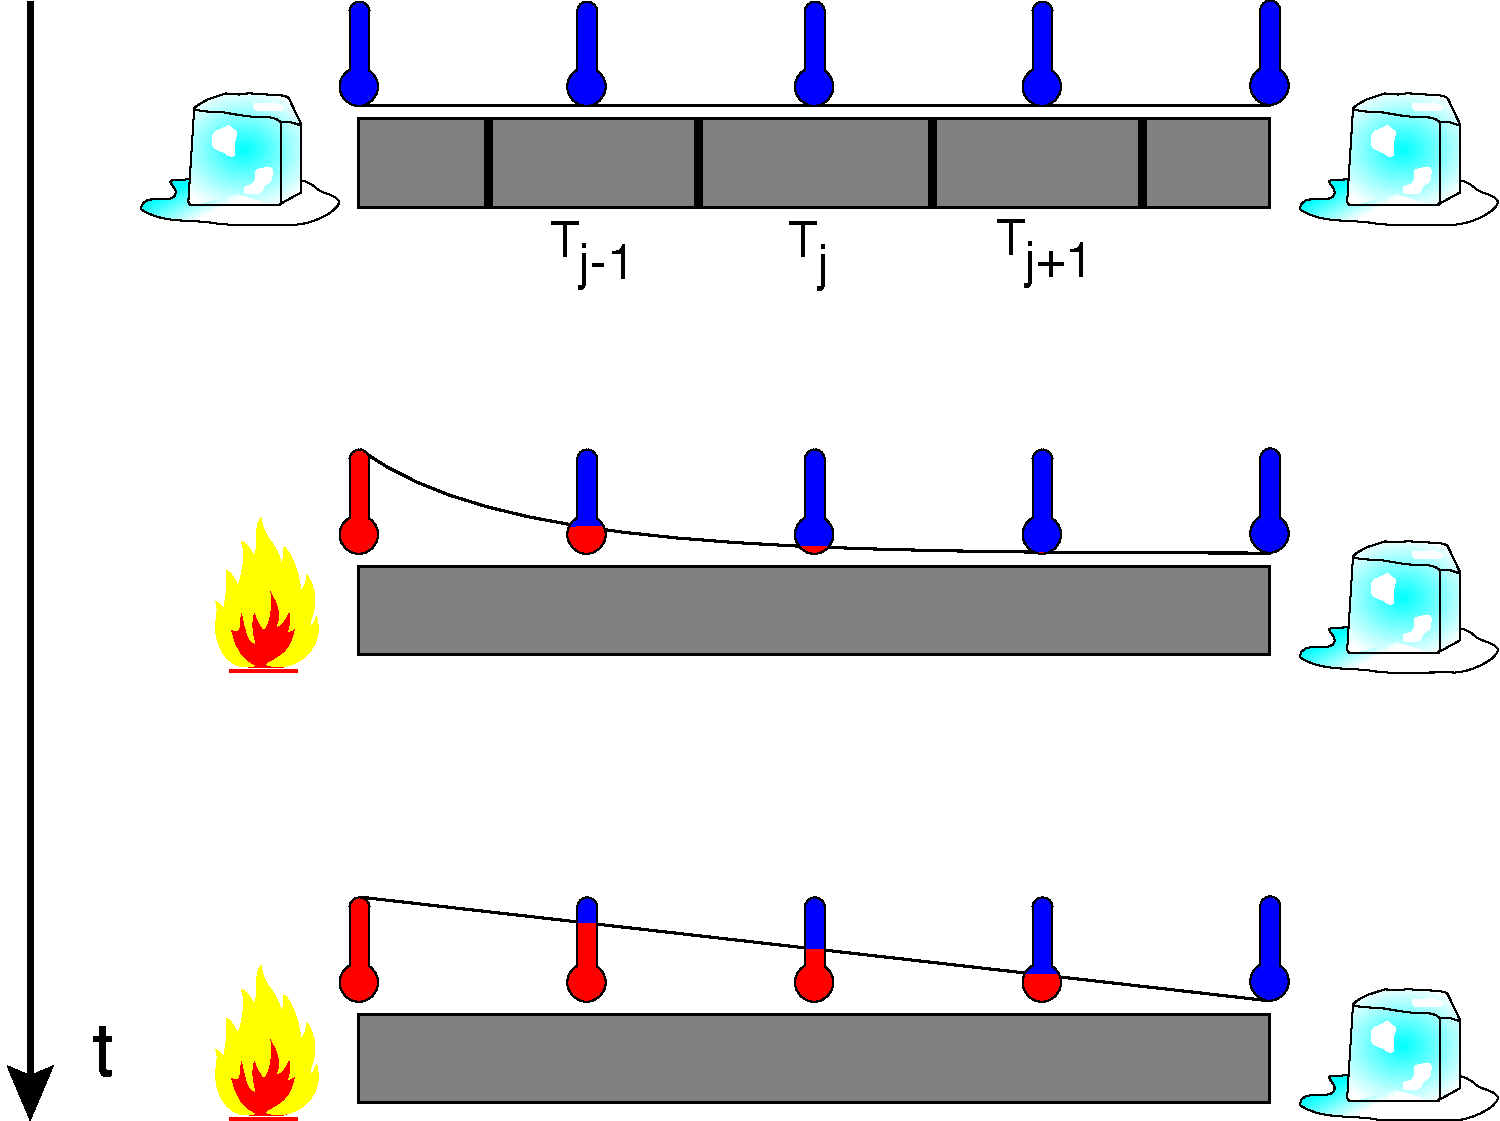
\includegraphics[width=5cm]{figures/heatconduction}%
   \\[.25em] \tiny{modified after \emph{Christophe Dang Ngoc Chan, wiki commons image}}
  \end{figure} 
    \column[c]{6.5cm}
  \begin{itemize}
  \item heat flows from \alert{higher} to \alert{lower} temperature
  \item this is the \alert{second law of thermodynamics}
 \begin{equation*}
    \mathbf{q} = -k \nabla T
  \end{equation*}
  \item the thermal conductivity $k$ is a measure for how fast the heat spreads
 \end{itemize}
  \end{columns}
\end{block}
\end{frame}


\section{Recap}

\begin{frame}
  \frametitle{Recap}
  \begin{block}{Balance Equations}
    \begin{equation*}
      \begin{array}{lrclc}
        \text{mass} \quad &  0& = & \nabla \cdot \mathbf{v} \quad & (1)\\[.25em]
        \text{momentum} \quad & \rho \frac{\text{d} \mathbf{v}}{\text{d} t} & = & -\nabla \cdot \mathbf{T'} + \nabla p + \mathbf{f} \quad & (3) \\[.25em]
        \text{temperature} \quad & \rho c\frac{\text{d} T}{\text{d} t} & = & - \nabla \cdot \mathbf{q} + \text{tr} \left(\mathbf{T}\cdot\mathbf{D}\right) + \rho r\quad & (1)
      \end{array}
    \end{equation*}
  \end{block}
  \begin{block}{Flow Law}
    \vskip-.5em
    \begin{equation*}
      \begin{array}{lrclc}
              \text{Glen's flow law}\quad & \mathbf{T}' & = & 2\,\eta\,\mathbf{D}  = A(T)^{-1/n}\sigma_{\text{e}}^{1-n}\mathbf{D} \quad &(6)
      \end{array}
    \end{equation*}
  \end{block}
  \begin{itemize}
  \item now we have 15 equations for 15 unknown fields
   \item the system is now well-determined
   \end{itemize}
 \end{frame}
 

\section{Glaciers}


\begin{frame}
  \frametitle{Large-Scale Dynamics}
  \begin{figure}
    \includegraphics<1| handout: 0>[width=7cm]{figures/fig_5_01}
    \includegraphics<2>[width=7cm]{figures/fig_5_01_sheet}
  \end{figure}
  \begin{itemize}
  \item Ice sheets are glaciers too!
  \item we will focus on the ice sheet part and, for now, ignore ice shelves
  \item ice is assumed to be incompressible, $\nabla \cdot \mathbf{v} = 0$
  \end{itemize}
\end{frame}

 
\section{Scale analysis}

\begin{frame}
  \frametitle{The Incompressible Navier-Stokes Equation}
  \begin{block}{Momentum Balance}
    \begin{equation}
        \underbrace{\rho \frac{\text{d} \mathbf{v}}{\text{d} t}}_{\text{acceleration}} = - \underbrace{\nabla \cdot \mathbf{T'}}_{\text{deviatoric}} + \underbrace{\nabla p}_{\text{isotropic}} + \underbrace{\rho\mathbf{g}}_{\text{gravity}} - \underbrace{2\rho\boldsymbol{\Omega} \times \mathbf{v}}_{\text{Coriolis force}} 
   \end{equation}
   This is the \alert{Navier-Stokes} equation for incompressible flow
   \vskip.5em
   \begin{itemize}
     \item still rather complicated
     \item do we really need all these terms?
     \item \alert{Scale Analysis} is a power- and useful concept to assess the relative importance of terms
     \end{itemize}
  \end{block}
\end{frame}
 
\begin{frame}
  \frametitle{Scale Analysis}
  \begin{block}{Some typical values for an ice sheet}
  \begin{equation*}
  \begin{array}{rccl}
    \text{horizontal extend} &  [L] & = & \unit{1000}\kilo\meter\\
    \text{vertical extend} & [H] & = & \unit{1}\kilo\meter \\
    \text{horizontal velocity} & [U] & = & \unit{100}\meter\power{a}{-1}\\
    \text{vertical velocity} & [W] & = & \unit{0.1}\meter\power{a}{-1}\\
    \text{pressure} & [P] & = & \rho g[H] = \unit{10}\mega\pascal\\
    \text{time-scale} & [T] & = &[L]/[U] = 10^{4}\usk\power{a}{1}\\
  \end{array}
  \end{equation*}
  \end{block}
  The aspect ratio $\epsilon$ is defined as
  \begin{equation*}
    \epsilon = \frac{[H]}{[L]} = \frac{[W]}{[L]} = 10^{-3} \text{ for an ice sheet}
  \end{equation*}
  \begin{itemize}
    \item The scaling argument for valley glaciers is almost the same
  \end{itemize}
\end{frame}


\begin{frame}
  \frametitle{Scale Analysis}
  \begin{block}{Froude number}
    The \alert{Froude number $Fr$} is the ratio of acceleration and pressure gradient. In the horizontal we have
  \begin{equation*}
    Fr = \frac{\rho[U]/[t]}{[P]/[L]} = \frac{\rho[U]^{2}/[L]}{\rho g [H]/[L]} = \frac{[U]^{2}}{g[H]} \approx 10^{-15}
  \end{equation*}
  and in the vertical
  \begin{equation*}
    Fr = \frac{\rho[W]/[t]}{[P]/[L]} = \frac{\rho[W]^{2}/[L]}{\rho g [H]/[L]} = \frac{[\epsilon U]^{2}}{g[H]} \approx 10^{-21}
  \end{equation*}
  $\Rightarrow$ The \alert{acceleration term} is \alert{negligible}
  \end{block}
\end{frame}


\begin{frame}
  \frametitle{Scale Analysis}
  \begin{block}{Rossby number}
    The \alert{Rossby number $Ro$} is the ratio of acceleration and Coriolis force
  \begin{equation*}
    Ro = \frac{\rho[U]/[t]}{2\rho\Omega[U]} = \frac{\rho[U]^{2}/[L]}{2\rho\Omega[U]} = \frac{[U]}{2 \Omega [L]} \approx 2\times10^{-8}
  \end{equation*}
  and thus the Coriolis to pressure gradient is
  \begin{equation*}
   \frac{2\rho\Omega[U]}{[P]/[L]} = \frac{Fr}{Ro}\approx 5 \times 10^{-8}
  \end{equation*}
  $\Rightarrow$ The \alert{Coriolis term} is also \alert{negligible}
  \end{block}
\end{frame}


\section{Stokes Equation}


\begin{frame}
  \frametitle{Stokes Equation}
  By neglecting both the
  \begin{itemize}
  \item acceleration term
  \item Coriolis term
  \end{itemize}
  the Navier-Stokes equation simplifies to
  \begin{eqnarray}
     \nabla \cdot \left(\eta\left(\nabla \mathbf{v} + \nabla \mathbf{v}^{\text{T}}\right)\right) - \nabla p & = & - \rho \mathbf{g}
  \end{eqnarray}
  \begin{itemize}
  \item gravitational force exerted on the ice is balanced by stress within the ice
  \item this is called the \alert{Stokes equation}
  \end{itemize}
\end{frame}


\section{Energy Balance}

\begin{frame}
  \frametitle{Temperature Equation}
  Recall the equation for temperature
  \begin{equation}
    \rho\frac{\text{d} T}{\text{d} t} = - \nabla \cdot \mathbf{q} + \text{tr} \left(\mathbf{T}\cdot\mathbf{D}\right) + \rho r
  \end{equation}
  \begin{itemize}
  \item except for the uppermost few centimeters of ice,\\ radiation is negligible
 \end{itemize}
  \begin{equation}
    \rho\frac{\text{d} T}{\text{d} t} = - \nabla \cdot \mathbf{q} + \text{tr} \left(\mathbf{T}\cdot\mathbf{D}\right)
  \end{equation}
\end{frame}



\section{Boundary Conditions}


\begin{frame}
  \frametitle{Boundary Conditions}
  \begin{block}{Balance Equations}
    \begin{equation*}
      \begin{array}{lrcl}
        \text{mass} \quad &  \nabla \cdot \mathbf{v}  & = & 0\\[.25em]
        \text{momentum} \quad &  \nabla \cdot \left(\eta\left(\nabla \mathbf{v} + \nabla \mathbf{v}^{\text{T}}\right)\right)- \nabla p & = &  -\rho\mathbf{g} \\[.25em]
        \text{temperature} \quad & \rho c\frac{\text{d} T}{\text{d} t} - \nabla \cdot \left(k \nabla T\right) & = &  \text{tr} \left(\mathbf{T}\cdot\mathbf{D}\right) 
      \end{array}
    \end{equation*}
  \end{block}
 \begin{block}{Boundary Conditions} 
  To solve this system of equations, we need boundary conditions:
  \begin{itemize}
  \item mass (kinematic)
  \item momentum (dynamic)
  \item temperature (thermodynamic)
  \end{itemize}
  \end{block}
\end{frame}



\begin{frame}
  \frametitle{Ice-Thickness Equation}
      \begin{beamercolorbox}[rounded=true,shadow=true]{boxed}
        \begin{eqnarray} \notag
     \frac{\partial H}{\partial t} &=& (\mathbf{q}_{\sf{in}} - \mathbf{q}_{\sf{out}}) + a_{s} - a_{b} \\[.5em]
      &=& - \nabla \cdot \mathbf{Q} + a_{s} - a_{b}
    \end{eqnarray}
  \end{beamercolorbox}
\begin{itemize}
  \item $ a_{s}$ and $a_{b}$ are in the vertical direction
  \item the volume flux $\mathbf{Q}$ is defined as
    \begin{equation*}
      \mathbf{Q} = 
      \left(
        \begin{array}{c}
          Q_x \\[.25em]
          Q_y
        \end{array}
      \right)
      =
      \left(
        \begin{array}{c}
          \int_{b}^{h} v_{x} \,\text{d} z \\[.25em]
          \int_{b}^{h} v_{y} \,\text{d} z
        \end{array}
      \right)
    \end{equation*}
  \item derivation on p. 70\,--\,72
  \item this is the central evolution equation in ice sheet dynamics
  \end{itemize}
\end{frame}





\begin{frame}
  \frametitle{Surface Dynamic Boundary Condition}
  Continuity of the stress vector
  \begin{equation}
    \mathbf{T}\cdot\mathbf{n} = \mathbf{T}_{\text{atm}}\cdot\mathbf{n}
  \end{equation}
  \begin{itemize}
  \item $\mathbf{T}_{\text{atm}}$ is the Cauchy stress tensor in the atmosphere
  \item atmospheric pressure and wind stress are small compared to stress in the ice
  \end{itemize}
  \begin{equation}
    \mathbf{T}\cdot\mathbf{n} = 0
  \end{equation}
  \begin{itemize}
  \item this is a \alert{stress-free condition}
  \end{itemize}
\end{frame}


\begin{frame}
  \frametitle{Basal Dynamic Boundary Condition}
  \begin{equation}
    \mathbf{T}\cdot\mathbf{n} = \mathbf{T}_{\text{lith}}\cdot\mathbf{n} 
  \end{equation}
  \begin{itemize}
  \item $\mathbf{T}_{\text{lith}}$ is the Cauchy stress tensor in the lithosphere
  \item unfortunately, we have no information about the stress state of the lithosphere
  \item this boundary condition is not very useful
  \item empirical relationship is required
  \item relate bed-parallel shear stress $\tau_{\text{b}}$ and bed-parallel basal velocity $u_{\text{b}}$
    \begin{equation*}
      u_{\text{b}} = f(\tau_{\text{b}})
    \end{equation*}
  \end{itemize}
\end{frame}


\begin{frame}
  \frametitle{Basal Dynamic Boundary Condition}
 \begin{itemize}
   \item we can distinguish two cases
     \begin{itemize}
     \item ice is frozen to the bed if temperature below pressure melting point $T_{\text{m}}$
     \item ice is sliding if temperature at pressure melting point $T_{\text{m}}$
     \end{itemize}
    \begin{equation*}
      u_{\text{b}} = \left\{
        \begin{array}{lcl}
          0, & T< T_{\text{m}} & \quad \text{Dirichlet condition}\\
          f(\tau_{\text{b}}), & T= T_{\text{m}} & \quad \text{Robin condition}
        \end{array}
        \right.
    \end{equation*}
    \item despite 50 years of work (and lots of progress), this remains one of the grand unsolved problems in glaciology
  \end{itemize}
\end{frame}

\begin{frame}
  \frametitle{Surface Thermodynamic Boundary Condition}
  \begin{itemize}
  \item the surface temperature  $T_{\text{s}}$ can be well approximated by the mean annual surface air temperature, as long as the latter is $\le
 0^{\circ}\,\text{C}$
 \item we therefore simply prescribe the surface temperature (Dirichlet condition):
 \end{itemize}
    \begin{equation*}
      T= T_{\text{s}} 
    \end{equation*}
\end{frame}


\begin{frame}
  \frametitle{Basal Thermodynamic Boundary Condition}
  \begin{block}{Cold Base}
    the heat flux into the ice equals the geothermal heat flux $q_{\text{geo}}^{\perp}$
    \begin{equation*}
      \mathbf{q} \cdot \mathbf{n} = q_{\text{geo}}^{\perp}
    \end{equation*}
  \end{block}
  \begin{block}{Temperate Base}
    the ice is at the pressure melting point $T_{\text{m}}$:
    \begin{equation*}
      T= T_{\text{m}} 
    \end{equation*}
  \end{block}
\end{frame}


\begin{frame}
  \frametitle{Thermomechanically-Coupled Glacier Flow}
  \begin{block}{Balance Equations}
    \footnotesize{
    \begin{equation*}
      \begin{array}{lrcl}
        \text{mass} \quad &  \nabla \cdot \mathbf{v}  & = & 0\\[.25em]
        \text{momentum} \quad &  \nabla \cdot \left(\eta\left(\nabla \mathbf{v} + \nabla \mathbf{v}^{\text{T}}\right)\right)- \nabla p & = &  -\rho\mathbf{g} \\[.25em]
        \text{temperature} \quad & \rho c\frac{\text{d} T}{\text{d} t} - \nabla \cdot \left(k \nabla T\right) & = &  \text{tr} \left(\mathbf{T}\cdot\mathbf{D}\right) 
      \end{array}
    \end{equation*}
  }
  \end{block}
 \begin{block}{Boundary Conditions} 
   \footnotesize{
    \begin{equation*}
      \begin{array}{lr}
        \text{mass} \quad &  
        \begin{array}{rl}
          \frac{\partial h}{\partial t} + v_{x}\frac{\partial h}{\partial x} + v_{y}\frac{\partial h}{\partial y} - v_{z} = a_{s} & \quad \text{surface} \\[.25em]
          \frac{\partial b}{\partial t} + v_{x}\frac{\partial b}{\partial x} + v_{y}\frac{\partial b}{\partial y} - v_{z} = a_{b} & \quad \text{base}
        \end{array}
        \\[1.25em]
        \text{momentum} \quad & 
        \begin{array}{rl}
          \mathbf{T}\cdot\mathbf{n} = 0 & \quad \text{surface} \\[.25em]
         u_{\text{b}} = \{0,f(\tau_{\text{b}})\} & \quad \text{base}
        \end{array}        
        \\[1.25em]
        \text{temperature} \quad & 
        \begin{array}{rl}
          T = T_{\text{s}} & \quad \text{surface} \\[.25em]
          T = T_{\text{m}} \quad  \text{or} \quad \mathbf{q} \cdot \mathbf{n} = q_{\text{geo}}^{\perp }& \quad \text{base}
        \end{array}
      \end{array}
    \end{equation*}
  }
 \end{block}
\end{frame}

\begin{frame}
  \frametitle{Numerical Modeling}
   \begin{itemize}
   \item the presented Stokes problem is solvable on a valley glacier scale
   \item but still very hard on a whole ice sheet scale
   \item for ice sheets, the shallowness (small aspect ratio) can be further exploited, this leads to a hierarchy of approximations
   \item Ed Bueler's Karthaus lecture is a good starting point
   \end{itemize}
\end{frame}
   


\appendix

\section{{Math Stuff}}

\begin{frame}
  \frametitle{Basics and Notation}
  \vskip-.25em
  \begin{itemize}
  \item  We assume a fixed orthonormal basis ${\mathbf{e}}_{x},{\mathbf{e}}_{y},{\mathbf{e}}_{z}$
  \item Einstein summation convention says that double indices (here $i$) imply summation
  \end{itemize}
  \begin{block}{Nabla}
    \begin{equation*}
      \nabla = {\mathbf{e}}_{x}\frac{\partial}{\partial x} +  {\mathbf{e}}_{y}\frac{\partial}{\partial y} +  {\mathbf{e}}_{z}\frac{\partial}{\partial z} =  {\mathbf{e}}_{i}\frac{\partial}{\partial x_{i}} 
    \end{equation*}
 \end{block}
  \begin{block}{Gradient}
   \begin{itemize}
   \item the gradient of the scalar quantity $g$ is thus
      \begin{equation*}
        \nabla g = {\mathbf{e}}_{x}\frac{\partial g}{\partial x} +  {\mathbf{e}}_{y}\frac{\partial g}{\partial y} +  {\mathbf{e}}_{z}\frac{\partial g}{\partial z} = \mathbf{e}_{i} g_{,i} =
        \left(
          \begin{array}{c}
            \partial g/\partial x\\
            \partial g/\partial y\\
            \partial g/\partial z
          \end{array}
        \right)
      \end{equation*}
    \end{itemize}
  \end{block}
\end{frame}
 
\begin{frame}
  \frametitle{Basics and Notation}
 \begin{block}{Divergence}
   \begin{itemize}
   \item the divergence of the quantity $\mathbf{g}$ is 
      \begin{equation*}
        \nabla \cdot \mathbf{g} = \frac{\partial g_{x}}{\partial x} + \frac{\partial g_{y}}{\partial y} + \frac{\partial g_{z}}{\partial z} = g_{i,i}
      \end{equation*}
    \end{itemize}
  \end{block}
 \begin{block}{Total Derivative}
   \begin{itemize}
   \item or \alert{material derivative} 
      \begin{equation*}
        \frac{\text{d} g}{\text{d} t} = \frac{\partial g}{\partial t} + \mathbf{v} \cdot \nabla g
     \end{equation*}
     \item where $\mathbf{v}$ is the velocity
    \end{itemize}
  \end{block}
\end{frame}
 
\begin{frame}
  \frametitle{Basics and Notation}
\begin{block}{Trace}
   \begin{itemize}
   \item the \alert{trace} of the n$\times$n matrix $\mathbf{A}$ is the sum of the diagonal elements
      \begin{equation*}
        \text{tr} \mathbf{A} = A_{11} + A_{22} + \ldots + A_{nn} = A_{ii}  
     \end{equation*}
    \end{itemize}
  \end{block}
\end{frame}

 \begin{frame}
  \frametitle{Recall from Vector Calculus}
  \vskip-.25em
  \begin{block}{Divergence Theorem}
    \begin{equation}
      \oint_{\partial \omega} \boldsymbol{\phi}\cdot \mathbf{n} \,\text{d}a = 
      \int_{\omega} \nabla \cdot \boldsymbol{\phi} \, \text{d} v
    \end{equation}
      \begin{itemize}
      \item The sum of all sources minus the sum of all sinks gives the net flow out of a region
     \end{itemize}
  \end{block}
  \begin{block}{Reynolds Transport Theorem}
    \begin{equation}
     \frac{\text{d}}{\text{d} t}\int_{\omega} \boldsymbol{\phi}\, \text{d} v =
     \int_{\omega} \frac{\partial \boldsymbol{\phi}}{\partial{t}} \, \text{d} v +
      \oint_{\partial \omega} \boldsymbol{\phi} \mathbf{v}\cdot\mathbf{n}\,\text{d}a 
    \end{equation}
      \begin{itemize}
     \item What was already there plus what goes in minus what goes out is what is there
      \end{itemize}
  \end{block}
\end{frame}


\begin{frame}
  \frametitle{The Cauchy Stress Tensor}
  \begin{columns}
    \column[c]{6cm}
    \begin{figure}
      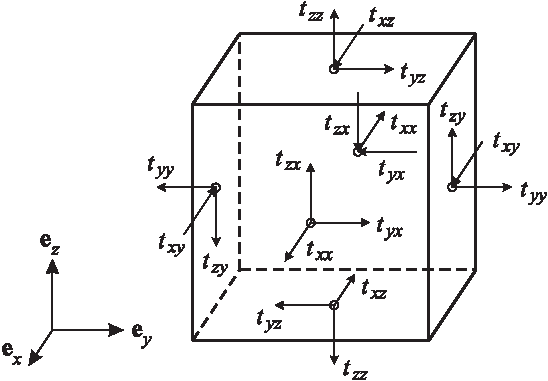
\includegraphics[width=5.cm]{figures/fig_3_08}
    \end{figure}
    \column[c]{5cm}
  \begin{displaymath} 
    \mathbf{T} = \left( 
      \begin{array}{ccc} 
        t_{xx} & t_{xy} & t_{xz} \\ 
        t_{yx} & t_{yy} & t_{yz} \\ 
        t_{zx} & t_{zx} & t_{zz} 
      \end{array} 
    \right) 
  \end{displaymath}
  \end{columns}
  \vskip1em
  For example
  \begin{displaymath}
    \mathbf{t}_{\mathbf{e}_{z}} =
    \left(
      \begin{array}{c}
        t_{xz}\\
        t_{yz}\\
        t_{zz}
      \end{array}
    \right)
  \end{displaymath}
  is the stress vector of a cut along the xy-plane
\end{frame}

\end{document}


